\documentclass[12 pt]{extarticle}

	\usepackage[frenchb]{babel}
	\usepackage[utf8]{inputenc}  
	\usepackage[T1]{fontenc}
	\usepackage{amssymb}
	\usepackage[mathscr]{euscript}
	\usepackage{stmaryrd}
	\usepackage{amsmath}
	\usepackage{tikz}
	\usepackage[all,cmtip]{xy}
	\usepackage{amsthm}
	\usepackage{varioref}
	\usepackage{geometry}
	\geometry{a4paper}
	\usepackage{lmodern}
	\usepackage{hyperref}
	\usepackage{array}
	 \usepackage{fancyhdr}
	 \usepackage{float}
	\pagestyle{fancy}
	\theoremstyle{plain}
	\fancyfoot[C]{\thepage} 
	\fancyhead[L]{Fiche d'exercices}
	\fancyhead[R]{2022-2023}
	
	
	\title{Exercices Chapitre 1}
	\date{}
	\begin{document}

\begin{center}{\Large Chapitre 2 - Proportionnalité}\\
 \end{center} 

\subsection*{Exercice 1}

Dans les tableaux suivants, reconnaître ceux qui sont des tableaux de proportionnalité. Pour ceux-là, donner le coefficient de proportionnalité. 

\begin{enumerate}
\item $
\begin{array}{|c|c|c|}
\hline
\phantom{000}    12    \phantom{000} 
& \phantom{000}    2   \phantom{000} & 
\phantom{000}
15
\phantom{000}\\
\hline

54 & 9  & 67,5\\
\hline
\end{array}$

\item $
\begin{array}{|c|c|c|}
\hline
\phantom{000}    22   \phantom{000} 
& \phantom{000}   27    \phantom{000} & 
\phantom{000}29
\phantom{000}\\
\hline
2 &7  & 9\\
\hline
\end{array}$

\item $
\begin{array}{|c|c|c|}
\hline
\phantom{000}    20    \phantom{000} 
& \phantom{000}     16  \phantom{000} & 
\phantom{000}
32
\phantom{000}\\
\hline

 15 & 12 & 24 \\
\hline
\end{array}$

\item $
\begin{array}{|c|c|c|}
\hline
\phantom{000}    2    \phantom{000} 
& \phantom{000}     5  \phantom{000} & 
\phantom{000}
7
\phantom{000}\\
\hline

4 & 25 & 49 \\
\hline
\end{array}$

\item $
\begin{array}{|c|c|c|}
\hline
\phantom{000}    10    \phantom{000} 
& \phantom{000}   13    \phantom{000} & 
\phantom{000}16
\phantom{000}\\
\hline
12 &15  & 18\\
\hline
\end{array}$

\item $
\begin{array}{|c|c|c|c|c|}
\hline
\phantom{000}     2   \phantom{000} 
& \phantom{000}    4   \phantom{000} 
& \phantom{000}    8   \phantom{000} 
& \phantom{000}    10 \phantom{000} 
& \phantom{000}   12    \phantom{000}\\
\hline
 7 & 14  &28 & 35 & 42 \\
\hline
\end{array}$

\item $
\begin{array}{|c|c|c|c|c|}
\hline
\phantom{000}    10    \phantom{000} 
& \phantom{000}    13   \phantom{000} 
& \phantom{000}      16 \phantom{000} 
& \phantom{000}      19 \phantom{000} 
& 
\phantom{000}
22
\phantom{000}\\
\hline

20 & 23 & 26& 29&32 \\
\hline
\end{array}$

\item $
\begin{array}{|c|c|c|c|c|}
\hline
\phantom{000}     3   \phantom{000} 
& \phantom{000}    4,5   \phantom{000} 
& \phantom{000}     9  \phantom{000} 
& \phantom{000}      10,5 \phantom{000} 
& 
\phantom{000}
15
\phantom{000}\\
\hline

 7& 10,5 &21 &24,5 & 35\\
\hline
\end{array}$
\end{enumerate}

\subsection*{Exercice 2}
Reprendre l'exercice précédent en plaçant les points sur un graphique pour chaque tableau et vérifier alors 
s'il y a proportionnalité sans calcul.
Vérifier qu'on obtient les mêmes réponses.
\subsection*{Exercice 3}

Remplir les tableaux de proportionnalité suivants : 

\begin{enumerate}
\item $
\begin{array}{|c|c|c|}
\hline
\phantom{000}     5   \phantom{000} 
& \phantom{000}       \phantom{000} & 
\phantom{000} 25
\phantom{000}\\
\hline
 7 &  84 & \\
\hline
\end{array}$

\item $
\begin{array}{|c|c|c|}
\hline
\phantom{000}    3    \phantom{000} 
& \phantom{000}     5  \phantom{000} & 
\phantom{000}
\phantom{000}\\
\hline
 & 123 & 369 \\
\hline
\end{array}$

\item $
\begin{array}{|c|c|c|}
\hline
\phantom{000}     12   \phantom{000} 
& \phantom{000}   18    \phantom{000} & 
\phantom{000}
30
\phantom{000}\\
\hline
 1696,8&  & 4242 \\
\hline
\end{array}$

\item $
\begin{array}{|c|c|c|c|c|}
\hline
\phantom{000}    7    \phantom{000} 
& \phantom{000}   21    \phantom{000} 
& \phantom{000}   35    \phantom{000} 
& \phantom{000}       \phantom{000} 
& 
\phantom{000}
77
\phantom{000}\\
\hline

 &39  & &104 & \\
\hline
\end{array}$

\item $
\begin{array}{|c|c|c|c|c|}
\hline
\phantom{000}        \phantom{000} 
& \phantom{000}       \phantom{000} 
& \phantom{000}     15  \phantom{000} 
& \phantom{000}      20 \phantom{000} 
& 
\phantom{000}
35
\phantom{000}\\
\hline

 10,2& 15,3 &25,5 & & \\
\hline
\end{array}$

\item $
\begin{array}{|c|c|c|c|c|}
\hline
\phantom{000}     12   \phantom{000} 
& \phantom{000}     32  \phantom{000} 
& \phantom{000}       \phantom{000} 
& \phantom{000}     84  \phantom{000} 
& 
\phantom{000}

\phantom{000}\\
\hline

 2,5 &  & 12,5 & &  25\\
\hline
\end{array}$
\end{enumerate}

\subsection*{Exercice 4}
Un avion réalise un vol Paris-Nice (900 kilomètres) en 1 heure et demie. 
\begin{enumerate}
\item Exprimer sa vitesse moyenne en kilomètres par heure, puis en kilomètres par minute. 
\item Combien de temps faudra-t-il au même avion pour effectuer un Paris-Rome (1100 kilomètres) ? Donner une durée exacte au format \_ heures \_ minutes. 
 
 \item Le même avion met $3$ heures et demie à aller de Paris à Athènes. En déduire la distance entre ces deux villes.  
\end{enumerate}

\subsection*{Exercice 5}
Le graphique suivant décrit la consommation en carburant d'un véhicule en fonction de la distance qu'il effectue.
\begin{figure}[H]
\center
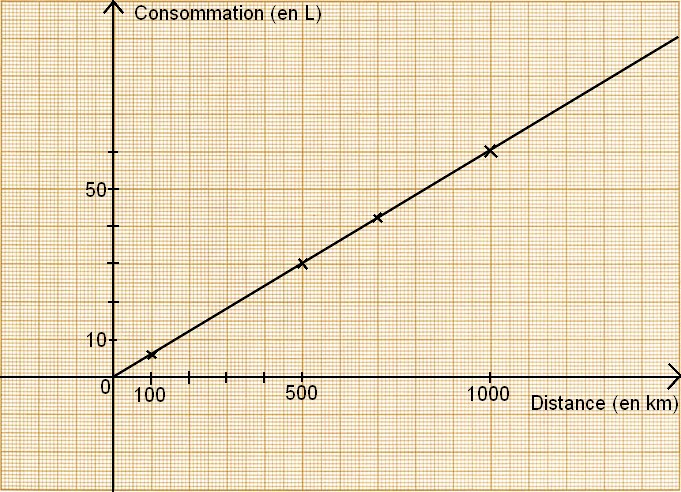
\includegraphics[scale=0.4]{Graphique}
\end{figure}

\begin{enumerate}
\item Est-on dans une situation de proportionnalité ?
\item Après 500 kilomètres, quel volume de carburant a été consommé ? 
\item Quelle distance peut-on parcourir avec 50 litres ?
\item On commence un trajet avec 60 litres d'essence, et on effectue 600 kilomètres. Peut-on faire le chemin de retour sans réapprovisionnement ? Si non, quelle quantité de carburant faudra-t-il racheter ?
\end{enumerate}

\subsection*{Exercice 6}

Un produit coûte 200 euros. 

\begin{enumerate}
\item Le vendeur propose d'abord une baisse de 10\%. Calculer le prix après cette réduction. 

\item Le prix remonte alors de 10\%. Calculer le nouveau prix, et le comparer au prix initial. 
\end{enumerate}

\subsection*{Exercice 7}

Un produit coûte 100 euros, et augmente de 3\% pendant 5 années consécutives. Calculer ses prix successifs. Exprimer l'augmentation totale en pourcentage du prix initial. 

\subsection*{Exercice 8}

Un produit coûte 10 euros en décembre.
\begin{enumerate}
\item On augmente le prix de 50\% en janvier, puis on revient au prix de départ en février . Exprimer la baisse de prix de février en pourcentage du prix de janvier.
\item On diminue le prix de 50\% en juin, puis on revient au prix de départ en juillet. 
Exprimer la hausse de prix en juillet en pourcentage du prix de juin.
\end{enumerate}

%\subsection*{Exercice 7}
%
%On rappelle qu'un mètre cube vaut $1000$ litres. La Marne a un débit moyen de 110 000 $L/s$. (En une seconde, 110 000 litres passent à travers une tranche donnée de la rivière.)
%
%\begin{enumerate}
%\item Exprimer ce débit en $m^3/s$.
%\item En prenant pour valeurs approximatives une profondeur moyenne de 6 mètres et une largeur de 70 mètres, calculer la section de la 
%rivière (c'est-à-dire sa surface si on la coupe de haut en bas et d'une rive à l'autre). 
%\item La vitesse du courant est donnée par le rapport du débit et de la section. Exprimer cette vitesse en mètres par seconde.
%
%
%\end{enumerate}
 	\end{document}
